\documentclass{article} % For LaTeX2e
\usepackage{iclr2019_conference,times}

% Optional math commands from https://github.com/goodfeli/dlbook_notation.
%%%%% NEW MATH DEFINITIONS %%%%%

\usepackage{amsmath,amsfonts,bm}

% Mark sections of captions for referring to divisions of figures
\newcommand{\figleft}{{\em (Left)}}
\newcommand{\figcenter}{{\em (Center)}}
\newcommand{\figright}{{\em (Right)}}
\newcommand{\figtop}{{\em (Top)}}
\newcommand{\figbottom}{{\em (Bottom)}}
\newcommand{\captiona}{{\em (a)}}
\newcommand{\captionb}{{\em (b)}}
\newcommand{\captionc}{{\em (c)}}
\newcommand{\captiond}{{\em (d)}}

% Highlight a newly defined term
\newcommand{\newterm}[1]{{\bf #1}}


% Figure reference, lower-case.
\def\figref#1{figure~\ref{#1}}
% Figure reference, capital. For start of sentence
\def\Figref#1{Figure~\ref{#1}}
\def\twofigref#1#2{figures \ref{#1} and \ref{#2}}
\def\quadfigref#1#2#3#4{figures \ref{#1}, \ref{#2}, \ref{#3} and \ref{#4}}
% Section reference, lower-case.
\def\secref#1{section~\ref{#1}}
% Section reference, capital.
\def\Secref#1{Section~\ref{#1}}
% Reference to two sections.
\def\twosecrefs#1#2{sections \ref{#1} and \ref{#2}}
% Reference to three sections.
\def\secrefs#1#2#3{sections \ref{#1}, \ref{#2} and \ref{#3}}
% Reference to an equation, lower-case.
\def\eqref#1{equation~\ref{#1}}
% Reference to an equation, upper case
\def\Eqref#1{Equation~\ref{#1}}
% A raw reference to an equation---avoid using if possible
\def\plaineqref#1{\ref{#1}}
% Reference to a chapter, lower-case.
\def\chapref#1{chapter~\ref{#1}}
% Reference to an equation, upper case.
\def\Chapref#1{Chapter~\ref{#1}}
% Reference to a range of chapters
\def\rangechapref#1#2{chapters\ref{#1}--\ref{#2}}
% Reference to an algorithm, lower-case.
\def\algref#1{algorithm~\ref{#1}}
% Reference to an algorithm, upper case.
\def\Algref#1{Algorithm~\ref{#1}}
\def\twoalgref#1#2{algorithms \ref{#1} and \ref{#2}}
\def\Twoalgref#1#2{Algorithms \ref{#1} and \ref{#2}}
% Reference to a part, lower case
\def\partref#1{part~\ref{#1}}
% Reference to a part, upper case
\def\Partref#1{Part~\ref{#1}}
\def\twopartref#1#2{parts \ref{#1} and \ref{#2}}

\def\ceil#1{\lceil #1 \rceil}
\def\floor#1{\lfloor #1 \rfloor}
\def\1{\bm{1}}
\newcommand{\train}{\mathcal{D}}
\newcommand{\valid}{\mathcal{D_{\mathrm{valid}}}}
\newcommand{\test}{\mathcal{D_{\mathrm{test}}}}

\def\eps{{\epsilon}}


% Random variables
\def\reta{{\textnormal{$\eta$}}}
\def\ra{{\textnormal{a}}}
\def\rb{{\textnormal{b}}}
\def\rc{{\textnormal{c}}}
\def\rd{{\textnormal{d}}}
\def\re{{\textnormal{e}}}
\def\rf{{\textnormal{f}}}
\def\rg{{\textnormal{g}}}
\def\rh{{\textnormal{h}}}
\def\ri{{\textnormal{i}}}
\def\rj{{\textnormal{j}}}
\def\rk{{\textnormal{k}}}
\def\rl{{\textnormal{l}}}
% rm is already a command, just don't name any random variables m
\def\rn{{\textnormal{n}}}
\def\ro{{\textnormal{o}}}
\def\rp{{\textnormal{p}}}
\def\rq{{\textnormal{q}}}
\def\rr{{\textnormal{r}}}
\def\rs{{\textnormal{s}}}
\def\rt{{\textnormal{t}}}
\def\ru{{\textnormal{u}}}
\def\rv{{\textnormal{v}}}
\def\rw{{\textnormal{w}}}
\def\rx{{\textnormal{x}}}
\def\ry{{\textnormal{y}}}
\def\rz{{\textnormal{z}}}

% Random vectors
\def\rvepsilon{{\mathbf{\epsilon}}}
\def\rvtheta{{\mathbf{\theta}}}
\def\rva{{\mathbf{a}}}
\def\rvb{{\mathbf{b}}}
\def\rvc{{\mathbf{c}}}
\def\rvd{{\mathbf{d}}}
\def\rve{{\mathbf{e}}}
\def\rvf{{\mathbf{f}}}
\def\rvg{{\mathbf{g}}}
\def\rvh{{\mathbf{h}}}
\def\rvu{{\mathbf{i}}}
\def\rvj{{\mathbf{j}}}
\def\rvk{{\mathbf{k}}}
\def\rvl{{\mathbf{l}}}
\def\rvm{{\mathbf{m}}}
\def\rvn{{\mathbf{n}}}
\def\rvo{{\mathbf{o}}}
\def\rvp{{\mathbf{p}}}
\def\rvq{{\mathbf{q}}}
\def\rvr{{\mathbf{r}}}
\def\rvs{{\mathbf{s}}}
\def\rvt{{\mathbf{t}}}
\def\rvu{{\mathbf{u}}}
\def\rvv{{\mathbf{v}}}
\def\rvw{{\mathbf{w}}}
\def\rvx{{\mathbf{x}}}
\def\rvy{{\mathbf{y}}}
\def\rvz{{\mathbf{z}}}

% Elements of random vectors
\def\erva{{\textnormal{a}}}
\def\ervb{{\textnormal{b}}}
\def\ervc{{\textnormal{c}}}
\def\ervd{{\textnormal{d}}}
\def\erve{{\textnormal{e}}}
\def\ervf{{\textnormal{f}}}
\def\ervg{{\textnormal{g}}}
\def\ervh{{\textnormal{h}}}
\def\ervi{{\textnormal{i}}}
\def\ervj{{\textnormal{j}}}
\def\ervk{{\textnormal{k}}}
\def\ervl{{\textnormal{l}}}
\def\ervm{{\textnormal{m}}}
\def\ervn{{\textnormal{n}}}
\def\ervo{{\textnormal{o}}}
\def\ervp{{\textnormal{p}}}
\def\ervq{{\textnormal{q}}}
\def\ervr{{\textnormal{r}}}
\def\ervs{{\textnormal{s}}}
\def\ervt{{\textnormal{t}}}
\def\ervu{{\textnormal{u}}}
\def\ervv{{\textnormal{v}}}
\def\ervw{{\textnormal{w}}}
\def\ervx{{\textnormal{x}}}
\def\ervy{{\textnormal{y}}}
\def\ervz{{\textnormal{z}}}

% Random matrices
\def\rmA{{\mathbf{A}}}
\def\rmB{{\mathbf{B}}}
\def\rmC{{\mathbf{C}}}
\def\rmD{{\mathbf{D}}}
\def\rmE{{\mathbf{E}}}
\def\rmF{{\mathbf{F}}}
\def\rmG{{\mathbf{G}}}
\def\rmH{{\mathbf{H}}}
\def\rmI{{\mathbf{I}}}
\def\rmJ{{\mathbf{J}}}
\def\rmK{{\mathbf{K}}}
\def\rmL{{\mathbf{L}}}
\def\rmM{{\mathbf{M}}}
\def\rmN{{\mathbf{N}}}
\def\rmO{{\mathbf{O}}}
\def\rmP{{\mathbf{P}}}
\def\rmQ{{\mathbf{Q}}}
\def\rmR{{\mathbf{R}}}
\def\rmS{{\mathbf{S}}}
\def\rmT{{\mathbf{T}}}
\def\rmU{{\mathbf{U}}}
\def\rmV{{\mathbf{V}}}
\def\rmW{{\mathbf{W}}}
\def\rmX{{\mathbf{X}}}
\def\rmY{{\mathbf{Y}}}
\def\rmZ{{\mathbf{Z}}}

% Elements of random matrices
\def\ermA{{\textnormal{A}}}
\def\ermB{{\textnormal{B}}}
\def\ermC{{\textnormal{C}}}
\def\ermD{{\textnormal{D}}}
\def\ermE{{\textnormal{E}}}
\def\ermF{{\textnormal{F}}}
\def\ermG{{\textnormal{G}}}
\def\ermH{{\textnormal{H}}}
\def\ermI{{\textnormal{I}}}
\def\ermJ{{\textnormal{J}}}
\def\ermK{{\textnormal{K}}}
\def\ermL{{\textnormal{L}}}
\def\ermM{{\textnormal{M}}}
\def\ermN{{\textnormal{N}}}
\def\ermO{{\textnormal{O}}}
\def\ermP{{\textnormal{P}}}
\def\ermQ{{\textnormal{Q}}}
\def\ermR{{\textnormal{R}}}
\def\ermS{{\textnormal{S}}}
\def\ermT{{\textnormal{T}}}
\def\ermU{{\textnormal{U}}}
\def\ermV{{\textnormal{V}}}
\def\ermW{{\textnormal{W}}}
\def\ermX{{\textnormal{X}}}
\def\ermY{{\textnormal{Y}}}
\def\ermZ{{\textnormal{Z}}}

% Vectors
\def\vzero{{\bm{0}}}
\def\vone{{\bm{1}}}
\def\vmu{{\bm{\mu}}}
\def\vtheta{{\bm{\theta}}}
\def\va{{\bm{a}}}
\def\vb{{\bm{b}}}
\def\vc{{\bm{c}}}
\def\vd{{\bm{d}}}
\def\ve{{\bm{e}}}
\def\vf{{\bm{f}}}
\def\vg{{\bm{g}}}
\def\vh{{\bm{h}}}
\def\vi{{\bm{i}}}
\def\vj{{\bm{j}}}
\def\vk{{\bm{k}}}
\def\vl{{\bm{l}}}
\def\vm{{\bm{m}}}
\def\vn{{\bm{n}}}
\def\vo{{\bm{o}}}
\def\vp{{\bm{p}}}
\def\vq{{\bm{q}}}
\def\vr{{\bm{r}}}
\def\vs{{\bm{s}}}
\def\vt{{\bm{t}}}
\def\vu{{\bm{u}}}
\def\vv{{\bm{v}}}
\def\vw{{\bm{w}}}
\def\vx{{\bm{x}}}
\def\vy{{\bm{y}}}
\def\vz{{\bm{z}}}

% Elements of vectors
\def\evalpha{{\alpha}}
\def\evbeta{{\beta}}
\def\evepsilon{{\epsilon}}
\def\evlambda{{\lambda}}
\def\evomega{{\omega}}
\def\evmu{{\mu}}
\def\evpsi{{\psi}}
\def\evsigma{{\sigma}}
\def\evtheta{{\theta}}
\def\eva{{a}}
\def\evb{{b}}
\def\evc{{c}}
\def\evd{{d}}
\def\eve{{e}}
\def\evf{{f}}
\def\evg{{g}}
\def\evh{{h}}
\def\evi{{i}}
\def\evj{{j}}
\def\evk{{k}}
\def\evl{{l}}
\def\evm{{m}}
\def\evn{{n}}
\def\evo{{o}}
\def\evp{{p}}
\def\evq{{q}}
\def\evr{{r}}
\def\evs{{s}}
\def\evt{{t}}
\def\evu{{u}}
\def\evv{{v}}
\def\evw{{w}}
\def\evx{{x}}
\def\evy{{y}}
\def\evz{{z}}

% Matrix
\def\mA{{\bm{A}}}
\def\mB{{\bm{B}}}
\def\mC{{\bm{C}}}
\def\mD{{\bm{D}}}
\def\mE{{\bm{E}}}
\def\mF{{\bm{F}}}
\def\mG{{\bm{G}}}
\def\mH{{\bm{H}}}
\def\mI{{\bm{I}}}
\def\mJ{{\bm{J}}}
\def\mK{{\bm{K}}}
\def\mL{{\bm{L}}}
\def\mM{{\bm{M}}}
\def\mN{{\bm{N}}}
\def\mO{{\bm{O}}}
\def\mP{{\bm{P}}}
\def\mQ{{\bm{Q}}}
\def\mR{{\bm{R}}}
\def\mS{{\bm{S}}}
\def\mT{{\bm{T}}}
\def\mU{{\bm{U}}}
\def\mV{{\bm{V}}}
\def\mW{{\bm{W}}}
\def\mX{{\bm{X}}}
\def\mY{{\bm{Y}}}
\def\mZ{{\bm{Z}}}
\def\mBeta{{\bm{\beta}}}
\def\mPhi{{\bm{\Phi}}}
\def\mLambda{{\bm{\Lambda}}}
\def\mSigma{{\bm{\Sigma}}}

% Tensor
\DeclareMathAlphabet{\mathsfit}{\encodingdefault}{\sfdefault}{m}{sl}
\SetMathAlphabet{\mathsfit}{bold}{\encodingdefault}{\sfdefault}{bx}{n}
\newcommand{\tens}[1]{\bm{\mathsfit{#1}}}
\def\tA{{\tens{A}}}
\def\tB{{\tens{B}}}
\def\tC{{\tens{C}}}
\def\tD{{\tens{D}}}
\def\tE{{\tens{E}}}
\def\tF{{\tens{F}}}
\def\tG{{\tens{G}}}
\def\tH{{\tens{H}}}
\def\tI{{\tens{I}}}
\def\tJ{{\tens{J}}}
\def\tK{{\tens{K}}}
\def\tL{{\tens{L}}}
\def\tM{{\tens{M}}}
\def\tN{{\tens{N}}}
\def\tO{{\tens{O}}}
\def\tP{{\tens{P}}}
\def\tQ{{\tens{Q}}}
\def\tR{{\tens{R}}}
\def\tS{{\tens{S}}}
\def\tT{{\tens{T}}}
\def\tU{{\tens{U}}}
\def\tV{{\tens{V}}}
\def\tW{{\tens{W}}}
\def\tX{{\tens{X}}}
\def\tY{{\tens{Y}}}
\def\tZ{{\tens{Z}}}


% Graph
\def\gA{{\mathcal{A}}}
\def\gB{{\mathcal{B}}}
\def\gC{{\mathcal{C}}}
\def\gD{{\mathcal{D}}}
\def\gE{{\mathcal{E}}}
\def\gF{{\mathcal{F}}}
\def\gG{{\mathcal{G}}}
\def\gH{{\mathcal{H}}}
\def\gI{{\mathcal{I}}}
\def\gJ{{\mathcal{J}}}
\def\gK{{\mathcal{K}}}
\def\gL{{\mathcal{L}}}
\def\gM{{\mathcal{M}}}
\def\gN{{\mathcal{N}}}
\def\gO{{\mathcal{O}}}
\def\gP{{\mathcal{P}}}
\def\gQ{{\mathcal{Q}}}
\def\gR{{\mathcal{R}}}
\def\gS{{\mathcal{S}}}
\def\gT{{\mathcal{T}}}
\def\gU{{\mathcal{U}}}
\def\gV{{\mathcal{V}}}
\def\gW{{\mathcal{W}}}
\def\gX{{\mathcal{X}}}
\def\gY{{\mathcal{Y}}}
\def\gZ{{\mathcal{Z}}}

% Sets
\def\sA{{\mathbb{A}}}
\def\sB{{\mathbb{B}}}
\def\sC{{\mathbb{C}}}
\def\sD{{\mathbb{D}}}
% Don't use a set called E, because this would be the same as our symbol
% for expectation.
\def\sF{{\mathbb{F}}}
\def\sG{{\mathbb{G}}}
\def\sH{{\mathbb{H}}}
\def\sI{{\mathbb{I}}}
\def\sJ{{\mathbb{J}}}
\def\sK{{\mathbb{K}}}
\def\sL{{\mathbb{L}}}
\def\sM{{\mathbb{M}}}
\def\sN{{\mathbb{N}}}
\def\sO{{\mathbb{O}}}
\def\sP{{\mathbb{P}}}
\def\sQ{{\mathbb{Q}}}
\def\sR{{\mathbb{R}}}
\def\sS{{\mathbb{S}}}
\def\sT{{\mathbb{T}}}
\def\sU{{\mathbb{U}}}
\def\sV{{\mathbb{V}}}
\def\sW{{\mathbb{W}}}
\def\sX{{\mathbb{X}}}
\def\sY{{\mathbb{Y}}}
\def\sZ{{\mathbb{Z}}}

% Entries of a matrix
\def\emLambda{{\Lambda}}
\def\emA{{A}}
\def\emB{{B}}
\def\emC{{C}}
\def\emD{{D}}
\def\emE{{E}}
\def\emF{{F}}
\def\emG{{G}}
\def\emH{{H}}
\def\emI{{I}}
\def\emJ{{J}}
\def\emK{{K}}
\def\emL{{L}}
\def\emM{{M}}
\def\emN{{N}}
\def\emO{{O}}
\def\emP{{P}}
\def\emQ{{Q}}
\def\emR{{R}}
\def\emS{{S}}
\def\emT{{T}}
\def\emU{{U}}
\def\emV{{V}}
\def\emW{{W}}
\def\emX{{X}}
\def\emY{{Y}}
\def\emZ{{Z}}
\def\emSigma{{\Sigma}}

% entries of a tensor
% Same font as tensor, without \bm wrapper
\newcommand{\etens}[1]{\mathsfit{#1}}
\def\etLambda{{\etens{\Lambda}}}
\def\etA{{\etens{A}}}
\def\etB{{\etens{B}}}
\def\etC{{\etens{C}}}
\def\etD{{\etens{D}}}
\def\etE{{\etens{E}}}
\def\etF{{\etens{F}}}
\def\etG{{\etens{G}}}
\def\etH{{\etens{H}}}
\def\etI{{\etens{I}}}
\def\etJ{{\etens{J}}}
\def\etK{{\etens{K}}}
\def\etL{{\etens{L}}}
\def\etM{{\etens{M}}}
\def\etN{{\etens{N}}}
\def\etO{{\etens{O}}}
\def\etP{{\etens{P}}}
\def\etQ{{\etens{Q}}}
\def\etR{{\etens{R}}}
\def\etS{{\etens{S}}}
\def\etT{{\etens{T}}}
\def\etU{{\etens{U}}}
\def\etV{{\etens{V}}}
\def\etW{{\etens{W}}}
\def\etX{{\etens{X}}}
\def\etY{{\etens{Y}}}
\def\etZ{{\etens{Z}}}

% The true underlying data generating distribution
\newcommand{\pdata}{p_{\rm{data}}}
% The empirical distribution defined by the training set
\newcommand{\ptrain}{\hat{p}_{\rm{data}}}
\newcommand{\Ptrain}{\hat{P}_{\rm{data}}}
% The model distribution
\newcommand{\pmodel}{p_{\rm{model}}}
\newcommand{\Pmodel}{P_{\rm{model}}}
\newcommand{\ptildemodel}{\tilde{p}_{\rm{model}}}
% Stochastic autoencoder distributions
\newcommand{\pencode}{p_{\rm{encoder}}}
\newcommand{\pdecode}{p_{\rm{decoder}}}
\newcommand{\precons}{p_{\rm{reconstruct}}}

\newcommand{\laplace}{\mathrm{Laplace}} % Laplace distribution

\newcommand{\E}{\mathbb{E}}
\newcommand{\Ls}{\mathcal{L}}
\newcommand{\R}{\mathbb{R}}
\newcommand{\emp}{\tilde{p}}
\newcommand{\lr}{\alpha}
\newcommand{\reg}{\lambda}
\newcommand{\rect}{\mathrm{rectifier}}
\newcommand{\softmax}{\mathrm{softmax}}
\newcommand{\sigmoid}{\sigma}
\newcommand{\softplus}{\zeta}
\newcommand{\KL}{D_{\mathrm{KL}}}
\newcommand{\Var}{\mathrm{Var}}
\newcommand{\standarderror}{\mathrm{SE}}
\newcommand{\Cov}{\mathrm{Cov}}
% Wolfram Mathworld says $L^2$ is for function spaces and $\ell^2$ is for vectors
% But then they seem to use $L^2$ for vectors throughout the site, and so does
% wikipedia.
\newcommand{\normlzero}{L^0}
\newcommand{\normlone}{L^1}
\newcommand{\normltwo}{L^2}
\newcommand{\normlp}{L^p}
\newcommand{\normmax}{L^\infty}

\newcommand{\parents}{Pa} % See usage in notation.tex. Chosen to match Daphne's book.

\DeclareMathOperator*{\argmax}{arg\,max}
\DeclareMathOperator*{\argmin}{arg\,min}

\DeclareMathOperator{\sign}{sign}
\DeclareMathOperator{\Tr}{Tr}
\let\ab\allowbreak


\usepackage{hyperref}
\usepackage{url}

\usepackage{algorithm}
\usepackage{algorithmic}
\usepackage{graphicx}
\graphicspath{{img/}}
\newcommand*\samethanks[1][\value{footnote}]{\footnotemark[#1]}


\title{AdaShift: Decorrelation and Convergence of Adaptive Learning Rate Methods \\ ICLR 2019 Reproducibility Challenge}

% Authors must not appear in the submitted version. They should be hidden
% as long as the \iclrfinalcopy macro remains commented out below.
% Non-anonymous submissions will be rejected without review.
% \newcommand*\samethanks[1][\value{footnote}]{\footnotemark[#1]}


\author{Mikhail Konobeev\thanks{Equal contribution}  \hspace{0.8mm}\samethanks[3] \hspace{0.8mm}, Irina Saparina\samethanks \hspace{1mm} \samethanks[3]  \hspace{1mm}, Taras Khakhulin\samethanks\hspace{1.5mm}\samethanks[2]\\
% \thanks{ Use footnote for providing further information
% about author (webpage, alternative address)---\emph{not} for acknowledging
% funding agencies.  Funding acknowledgements go at the end of the paper.} \\
% Department of Computer Science\\
Skolkovo Institute of Science and Technology\\
\samethanks[3]\hspace{1mm} National Research University Higher School of Economics \\
\samethanks[2]\hspace{1mm} Moscow Institute of Physics and Technology\\
\texttt{\{konobeeev.michael,irisaparina,t.khakhulin\}@gmail.com} }

% The \author macro works with any number of authors. There are two commands
% used to separate the names and addresses of multiple authors: \And and \AND.
%
% Using \And between authors leaves it to \LaTeX{} to determine where to break
% the lines. Using \AND forces a linebreak at that point. So, if \LaTeX{}
% puts 3 of 4 authors names on the first line, and the last on the second
% line, try using \AND instead of \And before the third author name.

\newcommand{\fix}{\marginpar{FIX}}
\newcommand{\new}{\marginpar{NEW}}

\iclrfinalcopy % Uncomment for camera-ready version, but NOT for submission.
\begin{document}


\maketitle

\begin{abstract}
AdaShift optimization method \citep{zhou2018adashift} attempts
to solve the problem of Adam by temporally and spatially
decorrelating momentum term and moving averages of squared
gradients. The method is proposed after an
analysis of Adam using net update factors that represent
the influence of the current gradient on the subsequent
optimization process and it was shown that decorrelating
moving averages of squared gradients with momentum terms
leads to balanced net update factors. In this work we
validate experimental results achieved by the authors
by reproducing them on top of PyTorch
\footnote{Our implementation is available online: \url{https://github.com/MichaelKonobeev/adashift}}. Overall, our
results agree with those reported by the authors, however we
find a small discrepancy between their implementation in TensorFlow
and description of the algorithm in the paper. Additionally,
we conduct more realistic experiments with generative model
and show that the proposed optimizer works in
a sequential online optimization problem on which Adam fails, even
though the problem does not meet the condition of gradients being
temporally independent.
\end{abstract}

\section{Introduction}

Adam \citep{kingma2014adam} is a popular optimization method
in deep learning as it uses only information about gradients
of the function being optimized and empirically achieves good
results in a variety of tasks. At the same time, it was noted that in some
problems it does not lead to convergence. \cite{reddi2018on}
provided an analysis of the issue and described a simple
optimization problem on which Adam fails.

The counterexample on which Adam fails is setup as an online
optimization problem in which some gradients have large
magnitude but occur rarely, while others have smaller
magnitude and are more frequent. It was argued that because of the
use of exponential moving average of squared past gradients
as an adaptive learning rate, the influence of gradients
with big magnitude disappears too quickly and the method
fails to converge. Proposed modifications
incorporated longer history of past squared gradients.

\cite{zhou2018adashift} analyzed Adam with proposed net update
factors that measure the impact of a current gradient on the
future optimization process. They show that in the sequential
online and stochastic optimization problems these net update
factors are unbalanced for Adam: gradients in the
right direction have smaller net update factors than
gradients in the wrong direction. It is
argued that the modification proposed by \cite{reddi2018on}
might not make the scaling factors very adaptive as it
consist of either increasing the weight of past squared gradients,
or taking element-wise maximum between the previous
squared scaling factor and a new value of exponential moving
average of squared gradients. It was further shown that
decorrelating scaling factors with the step direction
makes scaling factors balanced. The proposed AdaShift
method temporally shifts the scaling factor from the
step direction and uses an additional spacial function
that is applied to each block of parameters (such blocks
naturally occur in layers of deep neural networks).

In this work we describe our reproduction of the optimizer
and the experiments conducted by \cite{zhou2018adashift}
on top of PyTorch. Our results agree with those reported
by the authors. However, we
note a small discrepancy between authors implementation
and their description of the algorithm in the paper:
while in the paper spacial function is always applied before
squaring the gradients, in the code the gradients are
squared first. We use the same order as in the authors' code
in our experiments. As additional experiments,
we optimized the sequential online optimization problem
proposed by \cite{reddi2018on} and our results show
that AdaShift does converge to the correct point
even though as stated in the paper this optimization
problem does not meet the condition of gradients being temporally independent. We also train both discriminator
and generator in generative model WGAN-GP \citep{gulrajani2017improved} and report discriminator loss
and inception score.

% If your paper is ultimately accepted, the statement {\tt
%   {\textbackslash}iclrfinalcopy} should be inserted to adjust the
% format to the camera ready requirements.

% The format for the submissions is a variant of the NIPS format.
% Please read carefully the instructions below, and follow them
% faithfully.

\section{Preliminaries}\label{sec:preliminaries}

\paragraph{Adam.} General update rule for several common optimization
methods can be written in the following way:
\begin{equation}
    \theta_{t+1} \leftarrow \theta_t - \frac{\alpha_t}{
    \sqrt{v_t}}m_t,
\end{equation}
where $t$ is step number; $\theta_t \in \mathbb{R}^d$ is a vector of parameters; $\alpha_t$ is a learning rate;
$\sqrt{v_t} := \psi(g_1,\dots, g_t) \in\mathbb{R}_+^d$
is a scaling factor; and $m_t := \varphi(g_1,\dots, g_t)
\in\mathbb{R}^d$ is a function of historic gradients.
In Adam $m_t$ and $v_t$ are obtained from exponential moving averages. Firstly, consider
\begin{equation}
    m_t = \beta_1 m_{t - 1} + (1 - \beta_1) g_t,
    \qquad v_t = \beta_2 v_{t - 1} + (1 - \beta_2) g_t^2,
\end{equation}
where $\beta_1, \beta_2 \in [0, 1)$ are the exponential
decay rates for $m_t$ and $v_t$ respectively, and
$m_0 = v_0 = 0$.  These equations could be rewritten in the following way:
\begin{equation}
    m_t = (1 - \beta_1) \sum_{i = 1}^t \beta_1^{t - i} g_i,
    \qquad v_t = (1 - \beta_2) \sum_{i = 1}^t \beta_2^{t - i}
    g_i^2.
\end{equation}
\cite{kingma2014adam} also proposed implementing bias-correction
which leads to the following final equations:
\begin{equation}
    m_t = \frac{
    \sum_{i = 1}^t \beta_1^{t - i}g_i}{\sum_{i = 1}^t
    \beta_1^{t - i}},
    \qquad v_t = \frac{\sum_{i=1}^t \beta_2^{t - i}g_i^2}{
    \sum_{i=1}^t \beta_2^{t - i}}.
\end{equation}

\paragraph{Online optimization problem. } An online optimization
problem consists of a sequence of cost functions
$f_1(\theta), \dots, f_t(\theta), \dots, f_T(\theta)$. The performance of the optimizer is measured
using regret function $R(T) := \sum_{t=1}^T [f_t(\theta_t) -
f_t(\theta^*)]$, where $\theta^* := \arg\min_\theta
\sum_{t=1}^T f_t(\theta)$.

\paragraph{Counterexamples. }
For a fixed constants $d, C_1, C_2 \in \mathbb{N}$ such
that $C_1$ is sufficiently larger than
$C_2$ and a scalar parameter $\theta$ consider the
following sequential online optimization problem:
\begin{equation}\label{eq:sequential}
f_t(\theta) =  \begin{cases}
C_1\theta, & \text{if } t \text{ mod d} = 1; \\
-C_2\theta, & \text{otherwise.}
\end{cases}
\end{equation}
\cite{reddi2018on} additionally restricted the domain
of $f$ to $[-1, 1]$ which makes the optimum equal to -1.
However, Adam was show to converge to the value of 1.
Similarly, in stochastic optimization we consider the following $f_t$:
\begin{equation}\label{eq:stochastic}
    f_t(\theta) = \begin{cases}
    C\theta, & \text{with probability } p = \frac{1 + \delta}{C + 1};\\
    -\theta, & \text{with probability } 1 - p.
    \end{cases}
\end{equation}
Here optimum is attained at infinitely large negative value,
but Adam increases the value of the parameter.

\section{AdaShift: Decorrelation via Shifting}

\cite{zhou2018adashift} showed that the problem of
convergence on the synthetic counter examples stated
above could be solved by decorrelating $m_t$ and $v_t$.
This idea is implemented by temporarily shifting
gradients: the latest $n$ gradients are used to
compute the momentum term $m_t$ and older gradients
gradients are used to compute $v_t$. To further
decorrelate the two values, a function $\phi: \mathbb{R}^k
\rightarrow \mathbb{R}$ could be used. This function
is applied separately to each block of parameters where
a block corresponds to a kernel or a bias in a layer of
a network. In all of our experiments this function returns
the maximum value of a given vector unless stated otherwise. The pseudocode is presented in algorithm \ref{alg:adashift}.
In it we fix the order of taking squares of
the gradients and applying the function $\phi$:
the function is applied to squared gradients as in
the code provided by the authors and not the paper.
Our implementation has time complexity that is independent
of the number of kept gradients $n$ and
has linear space requirement in $n$.

\begin{algorithm}[t]
	\caption{AdaShift \citep{zhou2018adashift}}
	\label{alg:adashift}
	\begin{algorithmic}[1]
		\REQUIRE $n,\theta_0$, $g_0$, $\{f_t(\theta)\}^T_{t=1}$, $\{\alpha_t\}^T_{t=1}, \{g_i\}_{i=t-n + 1}^t, \beta_1, \beta_2$
		\STATE set $ v_0=0 $
		\FOR{$t=1$ \textbf{to} $T$}
	        \STATE $g_t = \nabla f_t(\theta_t)$
	        \STATE $m_t = \sum_{i=0}^{n - 1} \beta_1^i g_{t-i}/
	        \sum_{i = 0}^n\beta_1^i$
	        \STATE // Iterate over parameter blocks
    		\FOR{$i=1$ \textbf{to} $M$ }
        		\STATE $v_{t}[i] = \beta_2v_{t-1}[i] + (1-\beta_2)\phi(g^2_{t-1}[i])$
        		\STATE $v_t[i] = v_t[i] / (1 - \beta_2^t)$
        		\STATE $\theta_{t}[i]=\theta_{t-1}[i]- \alpha_t/\sqrt{v_{t}[i]} \cdot g_{t}[i]$
    		\ENDFOR
		\ENDFOR
	\end{algorithmic}
\end{algorithm}

\section{Experiments}
\subsection{Synthetic Examples}

We reproduce experiments on both of the synthetic examples and present the results in figure \ref{fig:synthetic}. In the stochastic online optimization problem the results
are comparable with those reported by the
authors: AdaShift moves the parameter in the right direction while also being faster than AMSGrad. Additionally, we note that
even on the sequential online optimization problem which
does not meet the requirement of gradients being temporarily
independent, AdaShift still converges to the optimal value of -1, even though it has larger regret than AMSGrad.

For sequential online optimization problem we set
the following values for the optimization problem parameters
$C_1 = 1010, C_2 = 10, d = 101$. The hyperparameters of the optimizers are  $\beta_1 = 0.9, \beta_2 = 0.99, \varepsilon = 0$, and the learning rate is
$\alpha_t = \alpha_0/\sqrt{t}$ where $\alpha_0=1$ and
$t$ is the iteration number. The number of kept gradients
$n$ is equal to 10. For stochastic
experiment use the same hyperparameters as the authors, namely, we set $C = 101, \delta = 0.002, \beta_1 = 0,
\beta_2 = 0.999$, $\alpha=10^{-3}$ without decay and
the number of kept gradients $n = 1$.

\begin{figure}[t]
    \centering
    \begin{minipage}{0.5\linewidth}
    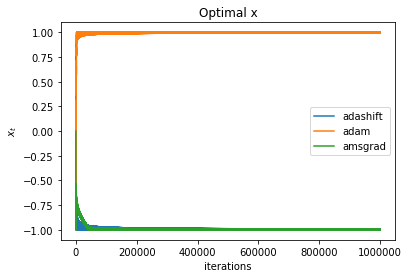
\includegraphics[width=0.99\linewidth]{opt_synth}
    \end{minipage}\hfill
    \begin{minipage}{0.5\linewidth}
    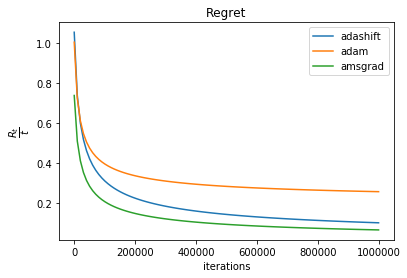
\includegraphics[width=0.99\linewidth]{regret_synth}
    \end{minipage}\\
    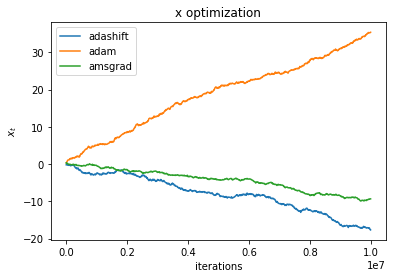
\includegraphics[width=0.5\linewidth]{synth-stochastic}
    \caption{Results on the synthetic examples described
    in section \ref{sec:preliminaries}. The plots on
    the top correspond to the sequential online optimization problem (\ref{eq:sequential}) (this experiment was not reported by the authors). The plot on the bottom corresponds to the stochastic optimization problem (\ref{eq:stochastic}). }\label{fig:synthetic}
\end{figure}

\subsection{MNIST}
During our verification of Logistic Regression and
Multilayer Perceptrion experiments on MNIST we use the
same experiment setup as the authors.
For Multilayer Perceptron we use two hidden layers with 256 hidden units  with no activation. We compare Adam, AMSGrad and AdaShift in two modes: with reduce-max spatial operation (max-AdaShift) and without spatial operation (non-AdaShift). For both models and all optimizers we set $\beta_1=0.0, \beta_2=0.999$; the learning rate for Adam, AMSGrad and  non-AdaShift was set to $0.001$, while for max-AdaShift it  was set to $0.01$. For AdaShift we use $n = 10$ latest gradients.
We train the models for 200 epochs with batch size equal to 64 as in the paper, but all methods converge in less than 10 epochs.

In figure \ref{fig:mnist:lr} we see that the results for Logistic Regression task for all methods  are very similar to each other and correspond to those reported in the paper. In the experiment with MLP we verify that non-AdaShift has higher training loss than other methods, but higher test accuracy. The results are noisy, so for the final plots we use smoothing in the same way as the authors.

\begin{figure}[t]
\centering
\begin{minipage}{.5\linewidth}
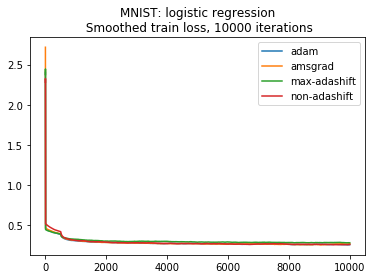
\includegraphics[width=.99\linewidth]{mnist_LR_smooth_1000.png}
\end{minipage}\hfill
\begin{minipage}{.5\linewidth}
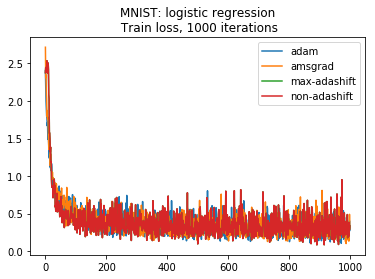
\includegraphics[width=.99\linewidth]{mnist_LR_1000.png}
\end{minipage}
\caption{Experiments with logistic regression on MNIST. Curves are smoothed by averaging over a window of fixed size.}\label{fig:mnist:lr}
\end{figure}

\begin{figure}[t]
\centering
\begin{minipage}{.5\linewidth}
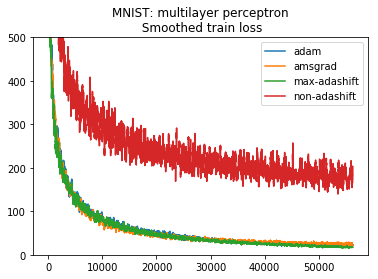
\includegraphics[width=.99\linewidth]{mnist_mlp.png}
\end{minipage}\hfill
\begin{minipage}{.5\linewidth}
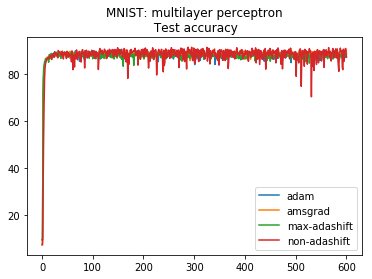
\includegraphics[width=.99\linewidth]{mlp_test_acc_mnist.png}
\end{minipage}
\caption{Experiments with MLP.}\label{fig:mnist:mlp}
\end{figure}

\subsubsection{WGAN-GP}

In this experiment we train discriminator with different
optimizers and use Adam for generator in WGAN-GP \citep{gulrajani2017improved}. In comparison,
authors only train discriminator against a fixed generator.

WGAN-GP uses Wasserstein distance as a measure of similarity between distributions: $W(p_r, p_g) = \inf_{\gamma \sim \Pi(p_r, p_g)} \mathbb{E}_{(x, y) \sim \gamma}[\| x-y \|]$. WGAN-GP penalizes the model if the gradient norm moves away from its target norm value 1 and the loss function for the discriminator is the following:
\begin{equation}\label{eq:wgan-gp}
L(p_r, p_g) = \max_{w \in W} \mathbb{E}_{x \sim p_r}[f_w(x)] - \mathbb{E}_{x \sim p_g}[f_w(x)] + \lambda \mathbb{E}_{x \sim p_x}[(\|\nabla f_w(x) \|_2 - 1)^2],
\end{equation}
where $\lambda$ is a penalty coefficient.
% Then the value of the target function for the discriminator closer to zero.
%, the W-distance less and discriminator can better distinguish generated images.

\begin{figure}[t]
\centering
\begin{minipage}{.5\linewidth}
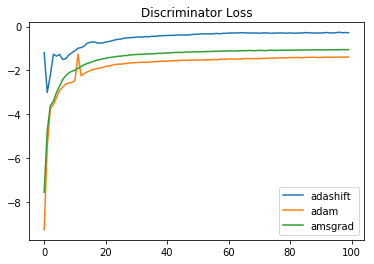
\includegraphics[width=.99\linewidth]{wgan-discriminator-loss.png}
\end{minipage}\hfill
\begin{minipage}{.5\linewidth}
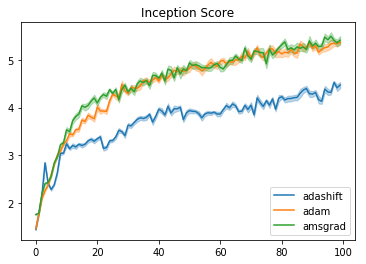
\includegraphics[width=.99\linewidth]{wgan-is.png}
\end{minipage}
\caption{Discriminator loss and Inception Score on the generative model WGAN-GP depending on epoch number. The first optimizer in label corresponds to discriminator and the second one to generator.}\label{fig:wgan}
\end{figure}

We report the discriminator loss and inception score
in figure \ref{fig:wgan}. From the figure it is noticeable
that for AdaShift the discriminator loss is higher during
training while the inception score is lower.  We also
trained a model in which both generator and discriminator
were optimized with different AdaShift optimizers but
it had worse inception score than the pair in which
AdaShift is used for discriminator and Adam is used for generator.

During training we make 5 discriminator iterations
per generator update and set learning rates to be constant
and equal to 2e-4 for all optimizers. The values of
exponential moving average rates are $\beta_1 = 0,
\beta_2 = 0.999$, batch size is $128$ and penalty
coefficient $\lambda$ is equal to 10.

We also attempted to reproduce the results reported by the authors.
In figure \ref{fig:wgan-fixed-generator} we report the discriminator
loss that is a modification of the loss (\ref{eq:wgan-gp}). For
this result we set batch size to 64, learning rates for Adam and AMSGrad equal to 1e-5 and learning rate for AdaShift to 2e-4. The penalty coefficient $\lambda$ is set to 0.1. We note that while in the paper Adam outperforms AMSGrad, in our experiment the converse is true. At the same time we confirm that AdaShift achieves the best result.

In this experiment, we note the atypical way in which the authors conducted their experiments with a generative model, specifically, by fixing generator and training only discriminator. Additionally, we note that the penalty coefficient significantly differed from the one used in the paper that proposed this method: authors set $\lambda$ to
0.1. We also note that authors use maxGP version of the loss function in their code. In our opinion, motivation and discussion of these choices would be beneficial.


\begin{figure}[t]
\centering
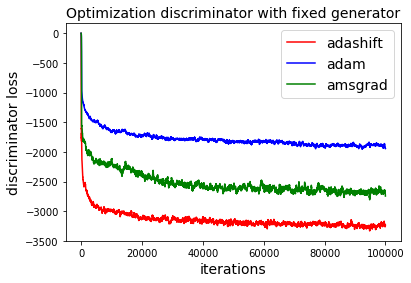
\includegraphics[width=.52\linewidth]{discriminator_fixed_gen.png}
\caption{WGAN-GP training discriminator against fixed generator. The curves are smoothed by averaging over a window of fixed size. }\label{fig:wgan-fixed-generator}
\end{figure}

\section{Neural Machine Translation}
\label{others}
We compare Adam, AMSGrad and AdaShift as optimizers for training Neural Machine Translation models. The authors use original implementation of GNMT \citep{luong17}, but it is available only in TensorFlow, so we add AMSGrad and AdaShift in OpenNMT-py system \citep{opennmt} and use it with similar parameters: we chose LSTM type of cells, bidirectional encoder, two layer in the encoder and the decoder; the size of hidden units and embeddings is 512 and we use Luong attention. For the inference we use beam-search with the size 10. We test the system on IWSLT-15 dataset with Vietnames as the source language  and English as the target. For all methods we use $\beta_1=0.0, \beta_2=0.9$, the learning rate for Adam, AMSGrad was $0.0001$, for max-AdaShift  the learning rate  was $0.01$. For AdaShift we use $n = 40$ kept gradients and we notice that with the default value $n = 10$ as used in the previous experiments, training procedure does not converge. Additionally, we decided to test Adam optimizer with $\beta_1=0.9, \beta_2=0.999$, because this setting is more realistic for NMT. In figure \ref{fig:nmt}
it could be seen that while with these hyperparameters
Adam does work better, its performance is still
significantly worse than that of AdaShift.

\begin{figure}[t]
\centering
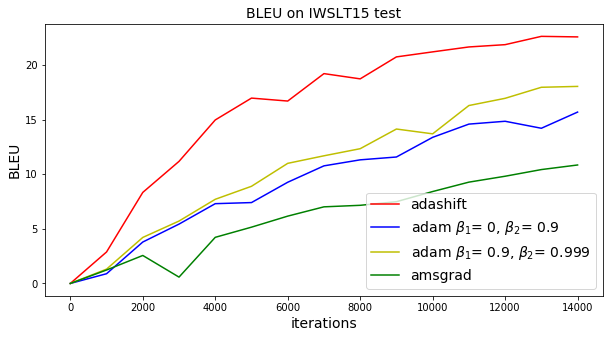
\includegraphics[width=.65\linewidth]{img/nmt_adam.png}
\caption{Results on the neural machine translation with seq2seq model.}
\label{fig:nmt}
\end{figure}

As we can see on the figure \ref{fig:nmt}  AdaShift achieves the best result in terms of BLEU score and converges faster than other methods. The results in the paper are similar to ours, but the curves are not exactly the same as in our experiments. The reason can be slight difference in NMT frameworks. It is not clear how many iterations authors used, because on the plot they also have 15000 iterations, but in the code they train the system with 30000 iterations. Our results are similar to theirs with 15000 iterations.

\section{Conclusion}
In this work we reproduced most of the experiments from the paper and confirmed that AdaShift i) fixes the problem
with Adam convergence ii) can outperform other
optimizers such as Adam and AMSGrad.
We found that in most tasks the proposed method is an efficient and easy way to stabilize the training process.  %However, it is worth noting that the authors did not have the theoretical guarantees for the convergence of this method so further work could be conducted in order to establish convergence guarantees.
We conducted more realistic experiment with generative models and although in our experiment with WGAN-GP task Wasserstein distance was close to zero with AdaShift, the quality of the generated images was worse than with other optimizers according to the inception score.
Experiment with NMT model shows that AdaShift can be the best option in a translation task. Overall, we conclude that AdaShift is a viable alternative to other optimization methods and that it can outperform them significantly on some tasks while solving the convergence problem of Adam.

\bibliography{iclr2019_conference}
\bibliographystyle{iclr2019_conference}

\end{document}
